\documentclass[twoside]{book}

% Packages required by doxygen
\usepackage{fixltx2e}
\usepackage{calc}
\usepackage{doxygen}
\usepackage[export]{adjustbox} % also loads graphicx
\usepackage{graphicx}
\usepackage[utf8]{inputenc}
\usepackage{makeidx}
\usepackage{multicol}
\usepackage{multirow}
\PassOptionsToPackage{warn}{textcomp}
\usepackage{textcomp}
\usepackage[nointegrals]{wasysym}
\usepackage[table]{xcolor}

% Font selection
\usepackage[T1]{fontenc}
\usepackage[scaled=.90]{helvet}
\usepackage{courier}
\usepackage{amssymb}
\usepackage{sectsty}
\renewcommand{\familydefault}{\sfdefault}
\allsectionsfont{%
  \fontseries{bc}\selectfont%
  \color{darkgray}%
}
\renewcommand{\DoxyLabelFont}{%
  \fontseries{bc}\selectfont%
  \color{darkgray}%
}
\newcommand{\+}{\discretionary{\mbox{\scriptsize$\hookleftarrow$}}{}{}}

% Page & text layout
\usepackage{geometry}
\geometry{%
  a4paper,%
  top=2.5cm,%
  bottom=2.5cm,%
  left=2.5cm,%
  right=2.5cm%
}
\tolerance=750
\hfuzz=15pt
\hbadness=750
\setlength{\emergencystretch}{15pt}
\setlength{\parindent}{0cm}
\setlength{\parskip}{3ex plus 2ex minus 2ex}
\makeatletter
\renewcommand{\paragraph}{%
  \@startsection{paragraph}{4}{0ex}{-1.0ex}{1.0ex}{%
    \normalfont\normalsize\bfseries\SS@parafont%
  }%
}
\renewcommand{\subparagraph}{%
  \@startsection{subparagraph}{5}{0ex}{-1.0ex}{1.0ex}{%
    \normalfont\normalsize\bfseries\SS@subparafont%
  }%
}
\makeatother

% Headers & footers
\usepackage{fancyhdr}
\pagestyle{fancyplain}
\fancyhead[LE]{\fancyplain{}{\bfseries\thepage}}
\fancyhead[CE]{\fancyplain{}{}}
\fancyhead[RE]{\fancyplain{}{\bfseries\leftmark}}
\fancyhead[LO]{\fancyplain{}{\bfseries\rightmark}}
\fancyhead[CO]{\fancyplain{}{}}
\fancyhead[RO]{\fancyplain{}{\bfseries\thepage}}
\fancyfoot[LE]{\fancyplain{}{}}
\fancyfoot[CE]{\fancyplain{}{}}
\fancyfoot[RE]{\fancyplain{}{\bfseries\scriptsize Generated by Doxygen }}
\fancyfoot[LO]{\fancyplain{}{\bfseries\scriptsize Generated by Doxygen }}
\fancyfoot[CO]{\fancyplain{}{}}
\fancyfoot[RO]{\fancyplain{}{}}
\renewcommand{\footrulewidth}{0.4pt}
\renewcommand{\chaptermark}[1]{%
  \markboth{#1}{}%
}
\renewcommand{\sectionmark}[1]{%
  \markright{\thesection\ #1}%
}

% Indices & bibliography
\usepackage{natbib}
\usepackage[titles]{tocloft}
\setcounter{tocdepth}{3}
\setcounter{secnumdepth}{5}
\makeindex

% Hyperlinks (required, but should be loaded last)
\usepackage{ifpdf}
\ifpdf
  \usepackage[pdftex,pagebackref=true]{hyperref}
\else
  \usepackage[ps2pdf,pagebackref=true]{hyperref}
\fi
\hypersetup{%
  colorlinks=true,%
  linkcolor=blue,%
  citecolor=blue,%
  unicode%
}

% Custom commands
\newcommand{\clearemptydoublepage}{%
  \newpage{\pagestyle{empty}\cleardoublepage}%
}

\usepackage{caption}
\captionsetup{labelsep=space,justification=centering,font={bf},singlelinecheck=off,skip=4pt,position=top}

%===== C O N T E N T S =====

\begin{document}

% Titlepage & ToC
\hypersetup{pageanchor=false,
             bookmarksnumbered=true,
             pdfencoding=unicode
            }
\pagenumbering{roman}
\begin{titlepage}
\vspace*{7cm}
\begin{center}%
{\Large My Project }\\
\vspace*{1cm}
{\large Generated by Doxygen 1.8.11}\\
\end{center}
\end{titlepage}
\clearemptydoublepage
\tableofcontents
\clearemptydoublepage
\pagenumbering{arabic}
\hypersetup{pageanchor=true}

%--- Begin generated contents ---
\chapter{Class Index}
\section{Class List}
Here are the classes, structs, unions and interfaces with brief descriptions\+:\begin{DoxyCompactList}
\item\contentsline{section}{\hyperlink{structnode}{node} }{\pageref{structnode}}{}
\item\contentsline{section}{\hyperlink{structnode1}{node1} }{\pageref{structnode1}}{}
\item\contentsline{section}{\hyperlink{structnode__info}{node\+\_\+info} }{\pageref{structnode__info}}{}
\end{DoxyCompactList}

\chapter{File Index}
\section{File List}
Here is a list of all files with brief descriptions\+:\begin{DoxyCompactList}
\item\contentsline{section}{\hyperlink{Lab1_8c}{Lab1.\+c} }{\pageref{Lab1_8c}}{}
\end{DoxyCompactList}

\chapter{Class Documentation}
\hypertarget{classCountMinSketch}{}\section{Count\+Min\+Sketch Class Reference}
\label{classCountMinSketch}\index{Count\+Min\+Sketch@{Count\+Min\+Sketch}}
\subsection*{Public Member Functions}
\begin{DoxyCompactItemize}
\item 
\hyperlink{classCountMinSketch_a0258a182a186433fc93ce136d566bb9f}{Count\+Min\+Sketch} (float ep, float gamm)
\item 
\hyperlink{classCountMinSketch_afd5fcf3bbe1ccbee00cd32ff605c96fc}{$\sim$\+Count\+Min\+Sketch} ()
\item 
void \hyperlink{classCountMinSketch_a3f6bcbf75a945ca7ccda17991ef145c3}{update} (int item, int c)
\item 
void \hyperlink{classCountMinSketch_acce9beb4ec1bb8ddb8d97eb4dfb74785}{update} (const char $\ast$str, int c)
\item 
\hyperlink{CountMinSketch_8cpp_a38190f0ee57a4f413c87037ad3bb91c6}{ui} \hyperlink{classCountMinSketch_a97b01c3251247d869ce75c37df6b778f}{estimate} (int item)
\item 
\hyperlink{CountMinSketch_8cpp_a38190f0ee57a4f413c87037ad3bb91c6}{ui} \hyperlink{classCountMinSketch_a4ca4e31be2f7ece94ce7a90ecc9da80c}{estimate} (const char $\ast$str)
\item 
\hyperlink{CountMinSketch_8cpp_a38190f0ee57a4f413c87037ad3bb91c6}{ui} \hyperlink{classCountMinSketch_a39170cd06d86f908cbb427a7f166b1e8}{totalcount} ()
\item 
\hyperlink{CountMinSketch_8cpp_a38190f0ee57a4f413c87037ad3bb91c6}{ui} \hyperlink{classCountMinSketch_ad60583d0353b1c5c10d927a66806da14}{hashstr} (const char $\ast$str)
\end{DoxyCompactItemize}
\subsection*{Private Member Functions}
\begin{DoxyCompactItemize}
\item 
void \hyperlink{classCountMinSketch_a3cbd681c7f2feef2927db7bb218db81b}{genajbj} (int $\ast$$\ast$\hyperlink{classCountMinSketch_abb764dbee3b01e8f35ee27c3ac71dc20}{hashes}, int i)
\end{DoxyCompactItemize}
\subsection*{Private Attributes}
\begin{DoxyCompactItemize}
\item 
\hyperlink{CountMinSketch_8cpp_a38190f0ee57a4f413c87037ad3bb91c6}{ui} \hyperlink{classCountMinSketch_a063b7a7097976a71f1eb112154977212}{w}
\item 
\hyperlink{CountMinSketch_8cpp_a38190f0ee57a4f413c87037ad3bb91c6}{ui} \hyperlink{classCountMinSketch_a385cf84231f967214bf6f71c6106f33e}{d}
\item 
float \hyperlink{classCountMinSketch_a71f4c0b4a1e3a75ab3f05c2774bf4ba8}{eps}
\item 
float \hyperlink{classCountMinSketch_ab7449c3f4d41400fb6104a3e62ac8126}{gamma}
\item 
\hyperlink{CountMinSketch_8cpp_a38190f0ee57a4f413c87037ad3bb91c6}{ui} \hyperlink{classCountMinSketch_a388d09d1902a17d772916eb289ef6306}{aj}
\item 
\hyperlink{CountMinSketch_8cpp_a38190f0ee57a4f413c87037ad3bb91c6}{ui} \hyperlink{classCountMinSketch_aededfa6cb03c61f49030320d5703e5ea}{bj}
\item 
\hyperlink{CountMinSketch_8cpp_a38190f0ee57a4f413c87037ad3bb91c6}{ui} \hyperlink{classCountMinSketch_a5a821d4e928c5d464b5388f78fc4f576}{total}
\item 
int $\ast$$\ast$ \hyperlink{classCountMinSketch_a6c911115ef4787d8825b7e2a39a64384}{C}
\item 
int $\ast$$\ast$ \hyperlink{classCountMinSketch_abb764dbee3b01e8f35ee27c3ac71dc20}{hashes}
\end{DoxyCompactItemize}


\subsection{Constructor \& Destructor Documentation}
\index{Count\+Min\+Sketch@{Count\+Min\+Sketch}!Count\+Min\+Sketch@{Count\+Min\+Sketch}}
\index{Count\+Min\+Sketch@{Count\+Min\+Sketch}!Count\+Min\+Sketch@{Count\+Min\+Sketch}}
\subsubsection[{\texorpdfstring{Count\+Min\+Sketch(float ep, float gamm)}{CountMinSketch(float ep, float gamm)}}]{\setlength{\rightskip}{0pt plus 5cm}Count\+Min\+Sketch\+::\+Count\+Min\+Sketch (
\begin{DoxyParamCaption}
\item[{float}]{ep, }
\item[{float}]{gamm}
\end{DoxyParamCaption}
)\hspace{0.3cm}{\ttfamily [inline]}}\hypertarget{classCountMinSketch_a0258a182a186433fc93ce136d566bb9f}{}\label{classCountMinSketch_a0258a182a186433fc93ce136d566bb9f}

\begin{DoxyCode}
35         \{
36             \textcolor{keywordflow}{if} (!(0.009 <= ep && ep < 1))
37             \{
38                 cout << \textcolor{stringliteral}{"eps must be in this range: [0.01, 1)"} << endl;
39                 exit(1);
40             \}
41             \textcolor{keywordflow}{else} \textcolor{keywordflow}{if} (!(0 < gamm && gamm < 1))
42             \{
43                 cout << \textcolor{stringliteral}{"gamma must be in this range: (0,1)"} << endl;
44                 exit(1);
45             \}
46             \hyperlink{classCountMinSketch_a71f4c0b4a1e3a75ab3f05c2774bf4ba8}{eps} = ep;
47             \hyperlink{classCountMinSketch_ab7449c3f4d41400fb6104a3e62ac8126}{gamma} = gamm;
48             \hyperlink{classCountMinSketch_a063b7a7097976a71f1eb112154977212}{w} = ceil(exp(1) / \hyperlink{classCountMinSketch_a71f4c0b4a1e3a75ab3f05c2774bf4ba8}{eps});
49             \hyperlink{classCountMinSketch_a385cf84231f967214bf6f71c6106f33e}{d} = ceil(log(1 / \hyperlink{classCountMinSketch_ab7449c3f4d41400fb6104a3e62ac8126}{gamma}));
50             \hyperlink{classCountMinSketch_a5a821d4e928c5d464b5388f78fc4f576}{total} = 0;
51             \hyperlink{classCountMinSketch_a6c911115ef4787d8825b7e2a39a64384}{C} = \textcolor{keyword}{new} \textcolor{keywordtype}{int} *[\hyperlink{classCountMinSketch_a385cf84231f967214bf6f71c6106f33e}{d}];
52             \hyperlink{CountMinSketch_8cpp_a38190f0ee57a4f413c87037ad3bb91c6}{ui} i, j;
53             \textcolor{keywordflow}{for} (i = 0; i < \hyperlink{classCountMinSketch_a385cf84231f967214bf6f71c6106f33e}{d}; i++)
54             \{
55                 \hyperlink{classCountMinSketch_a6c911115ef4787d8825b7e2a39a64384}{C}[i] = \textcolor{keyword}{new} \textcolor{keywordtype}{int}[\hyperlink{classCountMinSketch_a063b7a7097976a71f1eb112154977212}{w}];
56                 \textcolor{keywordflow}{for} (j = 0; j < \hyperlink{classCountMinSketch_a063b7a7097976a71f1eb112154977212}{w}; j++)
57                 \{
58                     \hyperlink{classCountMinSketch_a6c911115ef4787d8825b7e2a39a64384}{C}[i][j] = 0;
59                 \}
60             \}
61             srand(time(NULL));
62             \hyperlink{classCountMinSketch_abb764dbee3b01e8f35ee27c3ac71dc20}{hashes} = \textcolor{keyword}{new} \textcolor{keywordtype}{int}* [\hyperlink{classCountMinSketch_a385cf84231f967214bf6f71c6106f33e}{d}];
63             \textcolor{keywordflow}{for} (i = 0; i < \hyperlink{classCountMinSketch_a385cf84231f967214bf6f71c6106f33e}{d}; i++)
64             \{
65                 \hyperlink{classCountMinSketch_abb764dbee3b01e8f35ee27c3ac71dc20}{hashes}[i] = \textcolor{keyword}{new} \textcolor{keywordtype}{int}[2];
66                 \hyperlink{classCountMinSketch_a3cbd681c7f2feef2927db7bb218db81b}{genajbj}(\hyperlink{classCountMinSketch_abb764dbee3b01e8f35ee27c3ac71dc20}{hashes}, i);
67             \}
68         \}
\end{DoxyCode}
\index{Count\+Min\+Sketch@{Count\+Min\+Sketch}!````~Count\+Min\+Sketch@{$\sim$\+Count\+Min\+Sketch}}
\index{````~Count\+Min\+Sketch@{$\sim$\+Count\+Min\+Sketch}!Count\+Min\+Sketch@{Count\+Min\+Sketch}}
\subsubsection[{\texorpdfstring{$\sim$\+Count\+Min\+Sketch()}{~CountMinSketch()}}]{\setlength{\rightskip}{0pt plus 5cm}Count\+Min\+Sketch\+::$\sim$\+Count\+Min\+Sketch (
\begin{DoxyParamCaption}
{}
\end{DoxyParamCaption}
)\hspace{0.3cm}{\ttfamily [inline]}}\hypertarget{classCountMinSketch_afd5fcf3bbe1ccbee00cd32ff605c96fc}{}\label{classCountMinSketch_afd5fcf3bbe1ccbee00cd32ff605c96fc}

\begin{DoxyCode}
73         \{
74             \hyperlink{CountMinSketch_8cpp_a38190f0ee57a4f413c87037ad3bb91c6}{ui} i;
75             \textcolor{keywordflow}{for} (i = 0; i < \hyperlink{classCountMinSketch_a385cf84231f967214bf6f71c6106f33e}{d}; i++)
76             \{
77                 \textcolor{keyword}{delete}[] \hyperlink{classCountMinSketch_a6c911115ef4787d8825b7e2a39a64384}{C}[i];
78             \}
79             \textcolor{keyword}{delete}[] \hyperlink{classCountMinSketch_a6c911115ef4787d8825b7e2a39a64384}{C};
80             \textcolor{keywordflow}{for} (i = 0; i < \hyperlink{classCountMinSketch_a385cf84231f967214bf6f71c6106f33e}{d}; i++)
81             \{
82                 \textcolor{keyword}{delete}[] \hyperlink{classCountMinSketch_abb764dbee3b01e8f35ee27c3ac71dc20}{hashes}[i];
83             \}
84             \textcolor{keyword}{delete}[] \hyperlink{classCountMinSketch_abb764dbee3b01e8f35ee27c3ac71dc20}{hashes};
85         \}
\end{DoxyCode}


\subsection{Member Function Documentation}
\index{Count\+Min\+Sketch@{Count\+Min\+Sketch}!estimate@{estimate}}
\index{estimate@{estimate}!Count\+Min\+Sketch@{Count\+Min\+Sketch}}
\subsubsection[{\texorpdfstring{estimate(int item)}{estimate(int item)}}]{\setlength{\rightskip}{0pt plus 5cm}{\bf ui} Count\+Min\+Sketch\+::estimate (
\begin{DoxyParamCaption}
\item[{int}]{item}
\end{DoxyParamCaption}
)\hspace{0.3cm}{\ttfamily [inline]}}\hypertarget{classCountMinSketch_a97b01c3251247d869ce75c37df6b778f}{}\label{classCountMinSketch_a97b01c3251247d869ce75c37df6b778f}

\begin{DoxyCode}
112         \{
113             \textcolor{keywordtype}{int} minval = numeric\_limits<int>::max();
114             \textcolor{keywordtype}{unsigned} \textcolor{keywordtype}{int} hashval = NULL;
115             \textcolor{keywordflow}{for} (\textcolor{keywordtype}{unsigned} \textcolor{keywordtype}{int} j = 0; j < \hyperlink{classCountMinSketch_a385cf84231f967214bf6f71c6106f33e}{d}; j++)
116             \{
117                 hashval = (\hyperlink{classCountMinSketch_abb764dbee3b01e8f35ee27c3ac71dc20}{hashes}[j][0] * item + \hyperlink{classCountMinSketch_abb764dbee3b01e8f35ee27c3ac71dc20}{hashes}[j][1]) % \hyperlink{classCountMinSketch_a063b7a7097976a71f1eb112154977212}{w};
118                 minval = \hyperlink{CountMinSketch_8cpp_a3acffbd305ee72dcd4593c0d8af64a4f}{MIN}(minval, \hyperlink{classCountMinSketch_a6c911115ef4787d8825b7e2a39a64384}{C}[j][hashval]);
119             \}
120             \textcolor{keywordflow}{return} minval;
121         \}
\end{DoxyCode}
\index{Count\+Min\+Sketch@{Count\+Min\+Sketch}!estimate@{estimate}}
\index{estimate@{estimate}!Count\+Min\+Sketch@{Count\+Min\+Sketch}}
\subsubsection[{\texorpdfstring{estimate(const char $\ast$str)}{estimate(const char *str)}}]{\setlength{\rightskip}{0pt plus 5cm}{\bf ui} Count\+Min\+Sketch\+::estimate (
\begin{DoxyParamCaption}
\item[{const char $\ast$}]{str}
\end{DoxyParamCaption}
)\hspace{0.3cm}{\ttfamily [inline]}}\hypertarget{classCountMinSketch_a4ca4e31be2f7ece94ce7a90ecc9da80c}{}\label{classCountMinSketch_a4ca4e31be2f7ece94ce7a90ecc9da80c}

\begin{DoxyCode}
126         \{
127             \textcolor{keywordtype}{int} hashval = \hyperlink{classCountMinSketch_ad60583d0353b1c5c10d927a66806da14}{hashstr}(str);
128             \textcolor{keywordflow}{return} \hyperlink{classCountMinSketch_a97b01c3251247d869ce75c37df6b778f}{estimate}(hashval);
129         \}
\end{DoxyCode}
\index{Count\+Min\+Sketch@{Count\+Min\+Sketch}!genajbj@{genajbj}}
\index{genajbj@{genajbj}!Count\+Min\+Sketch@{Count\+Min\+Sketch}}
\subsubsection[{\texorpdfstring{genajbj(int $\ast$$\ast$hashes, int i)}{genajbj(int **hashes, int i)}}]{\setlength{\rightskip}{0pt plus 5cm}void Count\+Min\+Sketch\+::genajbj (
\begin{DoxyParamCaption}
\item[{int $\ast$$\ast$}]{hashes, }
\item[{int}]{i}
\end{DoxyParamCaption}
)\hspace{0.3cm}{\ttfamily [private]}}\hypertarget{classCountMinSketch_a3cbd681c7f2feef2927db7bb218db81b}{}\label{classCountMinSketch_a3cbd681c7f2feef2927db7bb218db81b}

\begin{DoxyCode}
157 \{
158     \hyperlink{classCountMinSketch_abb764dbee3b01e8f35ee27c3ac71dc20}{hashes}[i][0] = int(\textcolor{keywordtype}{float}(rand())*\textcolor{keywordtype}{float}(\hyperlink{CountMinSketch_8cpp_a550df3704559170eb0241ad9fb2af651}{LONG\_PRIME})/\textcolor{keywordtype}{float}(RAND\_MAX) + 1);
159     \hyperlink{classCountMinSketch_abb764dbee3b01e8f35ee27c3ac71dc20}{hashes}[i][1] = int(\textcolor{keywordtype}{float}(rand())*\textcolor{keywordtype}{float}(\hyperlink{CountMinSketch_8cpp_a550df3704559170eb0241ad9fb2af651}{LONG\_PRIME})/\textcolor{keywordtype}{float}(RAND\_MAX) + 1);
160 \}
\end{DoxyCode}
\index{Count\+Min\+Sketch@{Count\+Min\+Sketch}!hashstr@{hashstr}}
\index{hashstr@{hashstr}!Count\+Min\+Sketch@{Count\+Min\+Sketch}}
\subsubsection[{\texorpdfstring{hashstr(const char $\ast$str)}{hashstr(const char *str)}}]{\setlength{\rightskip}{0pt plus 5cm}{\bf ui} Count\+Min\+Sketch\+::hashstr (
\begin{DoxyParamCaption}
\item[{const char $\ast$}]{str}
\end{DoxyParamCaption}
)\hspace{0.3cm}{\ttfamily [inline]}}\hypertarget{classCountMinSketch_ad60583d0353b1c5c10d927a66806da14}{}\label{classCountMinSketch_ad60583d0353b1c5c10d927a66806da14}

\begin{DoxyCode}
142         \{
143             \textcolor{keywordtype}{unsigned} \textcolor{keywordtype}{long} hash = 5381;
144             \textcolor{keywordtype}{int} c;
145             \textcolor{keywordflow}{while} (c = *str++)
146             \{
147                 hash = ((hash << 5) + hash) + c;
148             \}
149             \textcolor{keywordflow}{return} hash;
150         \}
\end{DoxyCode}
\index{Count\+Min\+Sketch@{Count\+Min\+Sketch}!totalcount@{totalcount}}
\index{totalcount@{totalcount}!Count\+Min\+Sketch@{Count\+Min\+Sketch}}
\subsubsection[{\texorpdfstring{totalcount()}{totalcount()}}]{\setlength{\rightskip}{0pt plus 5cm}{\bf ui} Count\+Min\+Sketch\+::totalcount (
\begin{DoxyParamCaption}
{}
\end{DoxyParamCaption}
)\hspace{0.3cm}{\ttfamily [inline]}}\hypertarget{classCountMinSketch_a39170cd06d86f908cbb427a7f166b1e8}{}\label{classCountMinSketch_a39170cd06d86f908cbb427a7f166b1e8}

\begin{DoxyCode}
134         \{
135             \textcolor{keywordflow}{return} \hyperlink{classCountMinSketch_a5a821d4e928c5d464b5388f78fc4f576}{total};
136         \}
\end{DoxyCode}
\index{Count\+Min\+Sketch@{Count\+Min\+Sketch}!update@{update}}
\index{update@{update}!Count\+Min\+Sketch@{Count\+Min\+Sketch}}
\subsubsection[{\texorpdfstring{update(int item, int c)}{update(int item, int c)}}]{\setlength{\rightskip}{0pt plus 5cm}void Count\+Min\+Sketch\+::update (
\begin{DoxyParamCaption}
\item[{int}]{item, }
\item[{int}]{c}
\end{DoxyParamCaption}
)\hspace{0.3cm}{\ttfamily [inline]}}\hypertarget{classCountMinSketch_a3f6bcbf75a945ca7ccda17991ef145c3}{}\label{classCountMinSketch_a3f6bcbf75a945ca7ccda17991ef145c3}

\begin{DoxyCode}
90         \{
91             \hyperlink{classCountMinSketch_a5a821d4e928c5d464b5388f78fc4f576}{total} = \hyperlink{classCountMinSketch_a5a821d4e928c5d464b5388f78fc4f576}{total} + c;
92             \hyperlink{CountMinSketch_8cpp_a38190f0ee57a4f413c87037ad3bb91c6}{ui} hashval = NULL;
93             \textcolor{keywordflow}{for} (\hyperlink{CountMinSketch_8cpp_a38190f0ee57a4f413c87037ad3bb91c6}{ui} j = 0; j < \hyperlink{classCountMinSketch_a385cf84231f967214bf6f71c6106f33e}{d}; j++)
94             \{
95                 hashval = (\hyperlink{classCountMinSketch_abb764dbee3b01e8f35ee27c3ac71dc20}{hashes}[j][0] * item + \hyperlink{classCountMinSketch_abb764dbee3b01e8f35ee27c3ac71dc20}{hashes}[j][1]) % \hyperlink{classCountMinSketch_a063b7a7097976a71f1eb112154977212}{w};
96                 \hyperlink{classCountMinSketch_a6c911115ef4787d8825b7e2a39a64384}{C}[j][hashval] = \hyperlink{classCountMinSketch_a6c911115ef4787d8825b7e2a39a64384}{C}[j][hashval] + c;
97             \}
98         \}
\end{DoxyCode}
\index{Count\+Min\+Sketch@{Count\+Min\+Sketch}!update@{update}}
\index{update@{update}!Count\+Min\+Sketch@{Count\+Min\+Sketch}}
\subsubsection[{\texorpdfstring{update(const char $\ast$str, int c)}{update(const char *str, int c)}}]{\setlength{\rightskip}{0pt plus 5cm}void Count\+Min\+Sketch\+::update (
\begin{DoxyParamCaption}
\item[{const char $\ast$}]{str, }
\item[{int}]{c}
\end{DoxyParamCaption}
)\hspace{0.3cm}{\ttfamily [inline]}}\hypertarget{classCountMinSketch_acce9beb4ec1bb8ddb8d97eb4dfb74785}{}\label{classCountMinSketch_acce9beb4ec1bb8ddb8d97eb4dfb74785}

\begin{DoxyCode}
104         \{
105             \textcolor{keywordtype}{int} hashval = \hyperlink{classCountMinSketch_ad60583d0353b1c5c10d927a66806da14}{hashstr}(str);
106             \hyperlink{classCountMinSketch_a3f6bcbf75a945ca7ccda17991ef145c3}{update}(hashval, c);
107         \}
\end{DoxyCode}


\subsection{Member Data Documentation}
\index{Count\+Min\+Sketch@{Count\+Min\+Sketch}!aj@{aj}}
\index{aj@{aj}!Count\+Min\+Sketch@{Count\+Min\+Sketch}}
\subsubsection[{\texorpdfstring{aj}{aj}}]{\setlength{\rightskip}{0pt plus 5cm}{\bf ui} Count\+Min\+Sketch\+::aj\hspace{0.3cm}{\ttfamily [private]}}\hypertarget{classCountMinSketch_a388d09d1902a17d772916eb289ef6306}{}\label{classCountMinSketch_a388d09d1902a17d772916eb289ef6306}
\index{Count\+Min\+Sketch@{Count\+Min\+Sketch}!bj@{bj}}
\index{bj@{bj}!Count\+Min\+Sketch@{Count\+Min\+Sketch}}
\subsubsection[{\texorpdfstring{bj}{bj}}]{\setlength{\rightskip}{0pt plus 5cm}{\bf ui} Count\+Min\+Sketch\+::bj\hspace{0.3cm}{\ttfamily [private]}}\hypertarget{classCountMinSketch_aededfa6cb03c61f49030320d5703e5ea}{}\label{classCountMinSketch_aededfa6cb03c61f49030320d5703e5ea}
\index{Count\+Min\+Sketch@{Count\+Min\+Sketch}!C@{C}}
\index{C@{C}!Count\+Min\+Sketch@{Count\+Min\+Sketch}}
\subsubsection[{\texorpdfstring{C}{C}}]{\setlength{\rightskip}{0pt plus 5cm}int$\ast$$\ast$ Count\+Min\+Sketch\+::C\hspace{0.3cm}{\ttfamily [private]}}\hypertarget{classCountMinSketch_a6c911115ef4787d8825b7e2a39a64384}{}\label{classCountMinSketch_a6c911115ef4787d8825b7e2a39a64384}
\index{Count\+Min\+Sketch@{Count\+Min\+Sketch}!d@{d}}
\index{d@{d}!Count\+Min\+Sketch@{Count\+Min\+Sketch}}
\subsubsection[{\texorpdfstring{d}{d}}]{\setlength{\rightskip}{0pt plus 5cm}{\bf ui} Count\+Min\+Sketch\+::d\hspace{0.3cm}{\ttfamily [private]}}\hypertarget{classCountMinSketch_a385cf84231f967214bf6f71c6106f33e}{}\label{classCountMinSketch_a385cf84231f967214bf6f71c6106f33e}
\index{Count\+Min\+Sketch@{Count\+Min\+Sketch}!eps@{eps}}
\index{eps@{eps}!Count\+Min\+Sketch@{Count\+Min\+Sketch}}
\subsubsection[{\texorpdfstring{eps}{eps}}]{\setlength{\rightskip}{0pt plus 5cm}float Count\+Min\+Sketch\+::eps\hspace{0.3cm}{\ttfamily [private]}}\hypertarget{classCountMinSketch_a71f4c0b4a1e3a75ab3f05c2774bf4ba8}{}\label{classCountMinSketch_a71f4c0b4a1e3a75ab3f05c2774bf4ba8}
\index{Count\+Min\+Sketch@{Count\+Min\+Sketch}!gamma@{gamma}}
\index{gamma@{gamma}!Count\+Min\+Sketch@{Count\+Min\+Sketch}}
\subsubsection[{\texorpdfstring{gamma}{gamma}}]{\setlength{\rightskip}{0pt plus 5cm}float Count\+Min\+Sketch\+::gamma\hspace{0.3cm}{\ttfamily [private]}}\hypertarget{classCountMinSketch_ab7449c3f4d41400fb6104a3e62ac8126}{}\label{classCountMinSketch_ab7449c3f4d41400fb6104a3e62ac8126}
\index{Count\+Min\+Sketch@{Count\+Min\+Sketch}!hashes@{hashes}}
\index{hashes@{hashes}!Count\+Min\+Sketch@{Count\+Min\+Sketch}}
\subsubsection[{\texorpdfstring{hashes}{hashes}}]{\setlength{\rightskip}{0pt plus 5cm}int$\ast$$\ast$ Count\+Min\+Sketch\+::hashes\hspace{0.3cm}{\ttfamily [private]}}\hypertarget{classCountMinSketch_abb764dbee3b01e8f35ee27c3ac71dc20}{}\label{classCountMinSketch_abb764dbee3b01e8f35ee27c3ac71dc20}
\index{Count\+Min\+Sketch@{Count\+Min\+Sketch}!total@{total}}
\index{total@{total}!Count\+Min\+Sketch@{Count\+Min\+Sketch}}
\subsubsection[{\texorpdfstring{total}{total}}]{\setlength{\rightskip}{0pt plus 5cm}{\bf ui} Count\+Min\+Sketch\+::total\hspace{0.3cm}{\ttfamily [private]}}\hypertarget{classCountMinSketch_a5a821d4e928c5d464b5388f78fc4f576}{}\label{classCountMinSketch_a5a821d4e928c5d464b5388f78fc4f576}
\index{Count\+Min\+Sketch@{Count\+Min\+Sketch}!w@{w}}
\index{w@{w}!Count\+Min\+Sketch@{Count\+Min\+Sketch}}
\subsubsection[{\texorpdfstring{w}{w}}]{\setlength{\rightskip}{0pt plus 5cm}{\bf ui} Count\+Min\+Sketch\+::w\hspace{0.3cm}{\ttfamily [private]}}\hypertarget{classCountMinSketch_a063b7a7097976a71f1eb112154977212}{}\label{classCountMinSketch_a063b7a7097976a71f1eb112154977212}


The documentation for this class was generated from the following file\+:\begin{DoxyCompactItemize}
\item 
\hyperlink{CountMinSketch_8cpp}{Count\+Min\+Sketch.\+cpp}\end{DoxyCompactItemize}

\chapter{File Documentation}
\hypertarget{CountMinSketch_8cpp}{}\section{Count\+Min\+Sketch.\+cpp File Reference}
\label{CountMinSketch_8cpp}\index{Count\+Min\+Sketch.\+cpp@{Count\+Min\+Sketch.\+cpp}}
{\ttfamily \#include $<$iostream$>$}\\*
{\ttfamily \#include $<$cmath$>$}\\*
{\ttfamily \#include $<$map$>$}\\*
{\ttfamily \#include $<$cstdlib$>$}\\*
{\ttfamily \#include $<$ctime$>$}\\*
{\ttfamily \#include $<$limits$>$}\\*
{\ttfamily \#include $<$cstring$>$}\\*
Include dependency graph for Count\+Min\+Sketch.\+cpp\+:
\nopagebreak
\begin{figure}[H]
\begin{center}
\leavevmode
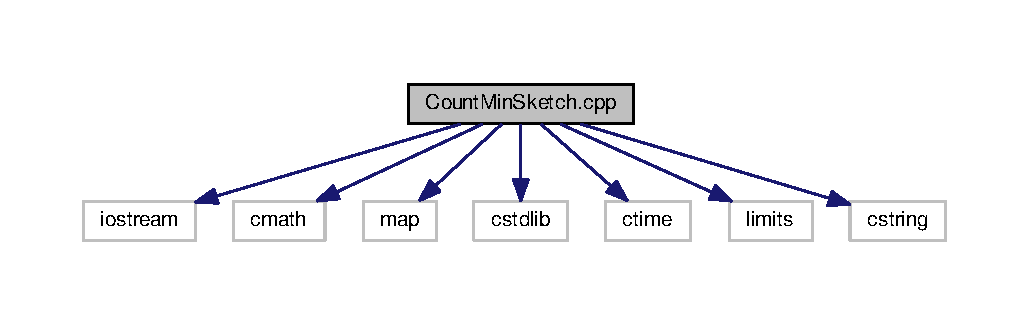
\includegraphics[width=350pt]{CountMinSketch_8cpp__incl}
\end{center}
\end{figure}
\subsection*{Classes}
\begin{DoxyCompactItemize}
\item 
class \hyperlink{classCountMinSketch}{Count\+Min\+Sketch}
\end{DoxyCompactItemize}
\subsection*{Macros}
\begin{DoxyCompactItemize}
\item 
\#define \hyperlink{CountMinSketch_8cpp_a550df3704559170eb0241ad9fb2af651}{L\+O\+N\+G\+\_\+\+P\+R\+I\+ME}~32993
\item 
\#define \hyperlink{CountMinSketch_8cpp_a3acffbd305ee72dcd4593c0d8af64a4f}{M\+IN}(a,  b)~(a $<$ b ? a \+: b)
\item 
\#define \hyperlink{CountMinSketch_8cpp_a38190f0ee57a4f413c87037ad3bb91c6}{ui}~unsigned int
\end{DoxyCompactItemize}
\subsection*{Functions}
\begin{DoxyCompactItemize}
\item 
int \hyperlink{CountMinSketch_8cpp_ae66f6b31b5ad750f1fe042a706a4e3d4}{main} ()
\end{DoxyCompactItemize}


\subsection{Macro Definition Documentation}
\index{Count\+Min\+Sketch.\+cpp@{Count\+Min\+Sketch.\+cpp}!L\+O\+N\+G\+\_\+\+P\+R\+I\+ME@{L\+O\+N\+G\+\_\+\+P\+R\+I\+ME}}
\index{L\+O\+N\+G\+\_\+\+P\+R\+I\+ME@{L\+O\+N\+G\+\_\+\+P\+R\+I\+ME}!Count\+Min\+Sketch.\+cpp@{Count\+Min\+Sketch.\+cpp}}
\subsubsection[{\texorpdfstring{L\+O\+N\+G\+\_\+\+P\+R\+I\+ME}{LONG_PRIME}}]{\setlength{\rightskip}{0pt plus 5cm}\#define L\+O\+N\+G\+\_\+\+P\+R\+I\+ME~32993}\hypertarget{CountMinSketch_8cpp_a550df3704559170eb0241ad9fb2af651}{}\label{CountMinSketch_8cpp_a550df3704559170eb0241ad9fb2af651}
\index{Count\+Min\+Sketch.\+cpp@{Count\+Min\+Sketch.\+cpp}!M\+IN@{M\+IN}}
\index{M\+IN@{M\+IN}!Count\+Min\+Sketch.\+cpp@{Count\+Min\+Sketch.\+cpp}}
\subsubsection[{\texorpdfstring{M\+IN}{MIN}}]{\setlength{\rightskip}{0pt plus 5cm}\#define M\+IN(
\begin{DoxyParamCaption}
\item[{}]{a, }
\item[{}]{b}
\end{DoxyParamCaption}
)~(a $<$ b ? a \+: b)}\hypertarget{CountMinSketch_8cpp_a3acffbd305ee72dcd4593c0d8af64a4f}{}\label{CountMinSketch_8cpp_a3acffbd305ee72dcd4593c0d8af64a4f}
\index{Count\+Min\+Sketch.\+cpp@{Count\+Min\+Sketch.\+cpp}!ui@{ui}}
\index{ui@{ui}!Count\+Min\+Sketch.\+cpp@{Count\+Min\+Sketch.\+cpp}}
\subsubsection[{\texorpdfstring{ui}{ui}}]{\setlength{\rightskip}{0pt plus 5cm}\#define ui~unsigned int}\hypertarget{CountMinSketch_8cpp_a38190f0ee57a4f413c87037ad3bb91c6}{}\label{CountMinSketch_8cpp_a38190f0ee57a4f413c87037ad3bb91c6}


\subsection{Function Documentation}
\index{Count\+Min\+Sketch.\+cpp@{Count\+Min\+Sketch.\+cpp}!main@{main}}
\index{main@{main}!Count\+Min\+Sketch.\+cpp@{Count\+Min\+Sketch.\+cpp}}
\subsubsection[{\texorpdfstring{main()}{main()}}]{\setlength{\rightskip}{0pt plus 5cm}int main (
\begin{DoxyParamCaption}
{}
\end{DoxyParamCaption}
)}\hypertarget{CountMinSketch_8cpp_ae66f6b31b5ad750f1fe042a706a4e3d4}{}\label{CountMinSketch_8cpp_ae66f6b31b5ad750f1fe042a706a4e3d4}

\begin{DoxyCode}
165 \{
166     \textcolor{keyword}{const} \textcolor{keywordtype}{char} *ar\_str[] = \{ \textcolor{stringliteral}{"hello"}, \textcolor{stringliteral}{"some"}, \textcolor{stringliteral}{"one"}, \textcolor{stringliteral}{"hello"}, \textcolor{stringliteral}{"alice"},
167                              \textcolor{stringliteral}{"one"}, \textcolor{stringliteral}{"lady"}, \textcolor{stringliteral}{"let"}, \textcolor{stringliteral}{"us"}, \textcolor{stringliteral}{"lady"},
168                              \textcolor{stringliteral}{"alice"}, \textcolor{stringliteral}{"in"}, \textcolor{stringliteral}{"us"}, \textcolor{stringliteral}{"wonderland"}, \textcolor{stringliteral}{"lady"},
169                              \textcolor{stringliteral}{"lady"}, \textcolor{stringliteral}{"some"}, \textcolor{stringliteral}{"hello"}, \textcolor{stringliteral}{"none"}, \textcolor{stringliteral}{"pie"} \};
170     \hyperlink{classCountMinSketch}{CountMinSketch} c(0.01, 0.1);
171     \hyperlink{CountMinSketch_8cpp_a38190f0ee57a4f413c87037ad3bb91c6}{ui} i, total = 0, count;
172     map<const char *, int> mapitems;
173     map<const char *, int>::const\_iterator it;
174     \textcolor{keywordflow}{for} (i = 0; i < 20; i++)
175     \{
176         \textcolor{keywordflow}{if} ((it = mapitems.find(ar\_str[i])) != mapitems.end())
177         \{
178             mapitems[ar\_str[i]] += i;
179         \}
180         \textcolor{keywordflow}{else}
181         \{
182             mapitems[ar\_str[i]] = i;
183         \}
184         c.update(ar\_str[i], i);
185         total = total + i;
186  
187     \}
188     \textcolor{comment}{// 1. test for items in ar\_str}
189     \textcolor{keywordflow}{for} (it = mapitems.begin(); it != mapitems.end(); it++)
190     \{
191         \textcolor{keywordflow}{if} (c.estimate(it->first) != mapitems[it->first])
192         \{
193             cout << \textcolor{stringliteral}{"Incorrect count for "} << it->first << \textcolor{stringliteral}{":->error: "};
194             count = abs(\textcolor{keywordtype}{int}(c.estimate(it->first)-mapitems[it->first]));
195             cout << count << endl;
196         \}
197         \textcolor{keywordflow}{else}
198         \{
199             cout << \textcolor{stringliteral}{"Correct count for '"} << it->first;
200             cout << \textcolor{stringliteral}{"' :-->count: "} << c.estimate(it->first) << endl;
201         \}
202     \}
203     cout << \textcolor{stringliteral}{"c.totalcount()==total ? "};
204     cout << (c.totalcount() == total ? \textcolor{stringliteral}{"True"} : \textcolor{stringliteral}{"False"}) << endl;
205     cout << \textcolor{stringliteral}{"Sketch Total: "} << c.totalcount() << endl;
206  
207     \textcolor{comment}{// 2. test for items not in ar\_str}
208     cout << \textcolor{stringliteral}{"Testing for strings not in ar\_str..."} << endl;
209     \textcolor{keyword}{const} \textcolor{keywordtype}{char} *arn\_str[] = \{\textcolor{stringliteral}{"sanfoundry"}, \textcolor{stringliteral}{"hello"}, \textcolor{stringliteral}{"linux"}, \textcolor{stringliteral}{"us"}\};
210     \textcolor{keywordflow}{for} (i = 0 ; i < 4; i++)
211     \{
212         \textcolor{keywordflow}{if} (!c.estimate(arn\_str[i]))
213             cout<<arn\_str[i] << \textcolor{stringliteral}{" not found in string array"}<<endl;
214         \textcolor{keywordflow}{else}
215             cout<<arn\_str[i] << \textcolor{stringliteral}{" found in string array"}<<endl;
216     \}
217     \textcolor{keywordflow}{return} 0;
218 \}\end{DoxyCode}


Here is the call graph for this function\+:
\nopagebreak
\begin{figure}[H]
\begin{center}
\leavevmode
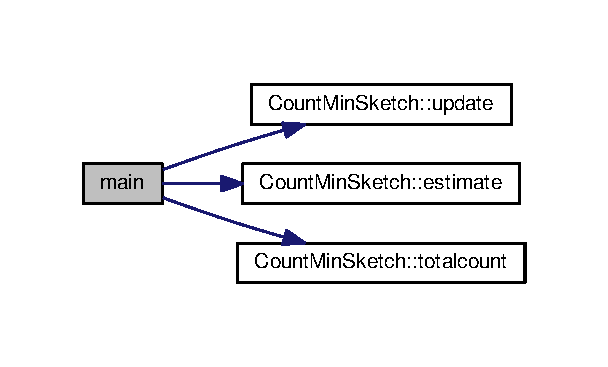
\includegraphics[width=292pt]{CountMinSketch_8cpp_ae66f6b31b5ad750f1fe042a706a4e3d4_cgraph}
\end{center}
\end{figure}



%--- End generated contents ---

% Index
\backmatter
\newpage
\phantomsection
\clearemptydoublepage
\addcontentsline{toc}{chapter}{Index}
\printindex

\end{document}
